\documentclass[conference]{IEEEtran}
\IEEEoverridecommandlockouts
% The preceding line is only needed to identify funding in the first footnote. If that is unneeded, please comment it out.
\usepackage[utf8]{inputenc}
\usepackage[spanish]{babel}
\usepackage{cite}
\usepackage{amsmath,amssymb,amsfonts}
\usepackage{algorithmic}
\usepackage{graphicx}
\usepackage{textcomp}
\usepackage{xcolor}
\usepackage{booktabs}
\usepackage{float}
\usepackage{listings}

% Configuración de estilo para código MATLAB
\lstdefinestyle{matlabstyle}{
    language=Matlab,
    basicstyle=\ttfamily\scriptsize,
    keywordstyle=\color{blue},
    commentstyle=\color{green!50!black},
    stringstyle=\color{red!70!black},
    numbers=left,
    numberstyle=\tiny\color{gray},
    numbersep=5pt,
    breaklines=true,
    breakatwhitespace=false,
    frame=single,
    rulecolor=\color{gray!40},
    showstringspaces=false,
    columns=fullflexible,
    keepspaces=true,
    captionpos=b
}



\def\BibTeX{{\rm B\kern-.05em{\sc i\kern-.025em b}\kern-.08em
    T\kern-.1667em\lower.7ex\hbox{E}\kern-.125emX}}
\begin{document}

\title{Estrategia de control basada en planitud diferencial para un sistema de doble péndulo invertido 
\thanks{Identify applicable funding agency here. If none, delete this.}
}

\author{\IEEEauthorblockN{Andrés Mauricio Morales Martínez}
\IEEEauthorblockA{\textit{Dept. Ingeniería Mecánica y Mecatrónica} \\
\textit{Universidad Nacional de Colombia }\\
Bogotá DC, Colombia \\
ORCID: 0009-0002-8353-1052}
\
}

\maketitle

\begin{abstract}
Este trabajo presenta el diseño y la evaluación de una estrategia de control basada en planitud diferencial para un sistema de doble péndulo invertido sobre un carro. A partir de una formulación energética, se deduce el modelo dinámico no lineal mediante el formalismo de Euler-Lagrange y se linealiza en torno al punto de equilibrio invertido. Del modelo lineal se obtiene la salida plana a través de la matriz de controlabilidad, lo que permite expresar el sistema en forma canónica controlable como una cadena de integradores. Se diseña entonces un controlador de seguimiento de trayectorias que combina la cancelación de la dinámica interna, la realimentación del error de estado y la prealimentación de la referencia, configurando la dinámica del error en lazo cerrado mediante ubicación de polos. Se comparan tres modelos desarrollados en Simulink (un modelo multicuerpo de referencia en Simscape, un modelo analítico no lineal y un modelo linealizado) para validar la formulación. El controlador se evalúa ante distintas condiciones iniciales y una perturbación externa. Los resultados confirman que el enfoque por salida plana permite un seguimiento y una estabilización efectivos en la vecindad del punto de operación, a la vez que evidencian las limitaciones propias de un diseño linealizado localmente al operar lejos del equilibrio.
\end{abstract}

\begin{IEEEkeywords}
component, formatting, style, styling, insert
\end{IEEEkeywords}

\section{Introducción}
El sistema de doble péndulo invertido es un problema clásico de control no lineal, empleado habitualmente como banco de pruebas (\textit{benchmark}) para validar nuevas estrategias de compensación. El sistema consiste en un carro al que se conectan dos articulaciones rotativas que permiten el movimiento libre de las masas pendulares. El objetivo de control consiste en mantener la posición invertida de ambos péndulos actuando únicamente sobre el desplazamiento horizontal del carro.\\

\begin{figure}
\center
	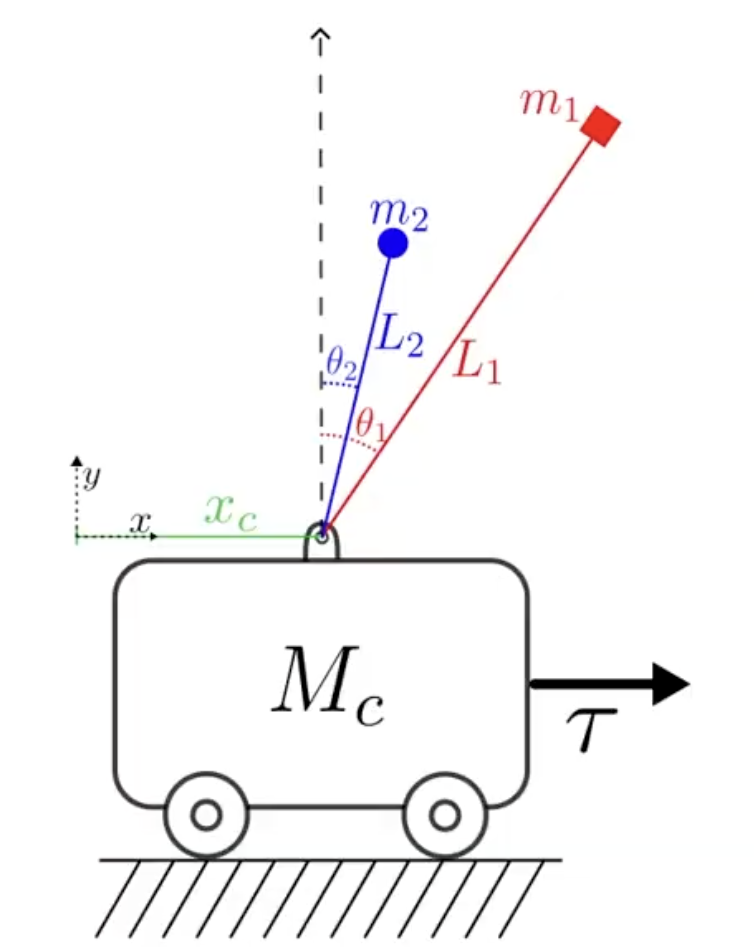
\includegraphics[width=0.5\linewidth]{imgs/modelo/modelo_mecanico.png}
	\caption{Sistema mecánico. Doble péndulo invertido sobre un carro con desplazamiento horizontal.}
\end{figure}
\\

Este sistema mecánico constituye una extensión del problema clásico del péndulo invertido. Para este último, suelen emplearse métodos como LQR o LQG como controladores de referencia. Sin embargo, la incorporación de un segundo péndulo aumenta considerablemente la dificultad del problema de control. En este contexto surge la planitud diferencial como herramienta matemática que permite expresar tanto la entrada de control como las salidas del sistema en función de una salida plana $z$ y de un número finito de sus derivadas:

\begin{equation}
	u = f(z, \dot{z}, \ddot{z}, \dots)
\end{equation}
\begin{equation}
	y = \phi(z, \dot{z}, \ddot{z}, \dots)
\end{equation}

Esta propiedad conduce a una dinámica descrita por una forma canónica controlable, lo que facilita considerablemente el diseño de una acción de control que satisfaga las especificaciones impuestas sobre el sistema. 

\section{Planteamiento matemático}
\subsection{Modelamiento dinámico Lagrangiano}
Se parte de un modelado energético basado en el formalismo de Lagrange. Se define el Lagrangiano $L$ como:  

\begin{equation}
	L = T - V
\end{equation}

El sistema posee tres grados de libertad. Se proponen las coordenadas generalizadas

\begin{equation}
	q = \begin{pmatrix}
		x_c & \theta_1 & \theta_2
	\end{pmatrix}^T \in \mathbb{R}^3,
\end{equation}

correspondientes a la posición del carro y a los ángulos de los péndulos respecto a la vertical, respectivamente.\\

Con ello, la energía cinética del sistema se expresa como 

\begin{equation}
	T = \frac{1}{2}M_c \dot{x}_c^2 + \frac{1}{2} m_1(\dot{x}_1^2 + \dot{y}_1^2) + \frac{1}{2} m_2(\dot{x}_2^2 + \dot{y}_2^2).
\end{equation}

Se imponen las restricciones de acoplamiento (ligaduras) 
\begin{equation}
	x_1 = x_c + l_1 \sin{\theta_1} \hspace{1cm} 	y_1= l_1 \cos{\theta_1}
\end{equation}
\begin{equation}
	x_2 = x_c + l_2 \sin{\theta_2} \hspace{1cm} 	y_2= l_2 \cos{\theta_2}
\end{equation}

La energía potencial se define como 

\begin{equation}
V_1 =	m_1 g l_1 \cos{\theta_1} \hspace{1cm} V_2 = m_2 g l_2 \cos{\theta_2}
\end{equation}

Con $V = V_1 + V_2$ y sustituyendo las ligaduras en los términos de $T$, es posible aplicar las ecuaciones de Euler--Lagrange \eqref{eq:euler} para obtener las ecuaciones de movimiento y, finalmente, el modelo dinámico del sistema:

\begin{equation}
	\frac{d}{dt}\left( \frac{\partial L}{\partial \dot{q}} \right) - \frac{\partial L}{\partial q}  = Q_i
	\label{eq:euler}
\end{equation}

\begin{equation}
M(q)\,\ddot{q} + d(q,\dot{q}) + G(q) = P_u
\end{equation}


La matriz de inercia está dada por

\begin{equation}
M(q)=
\begin{bmatrix}
M_c+m_1+m_2 &
m_1 l_1 \cos\theta_1 &
m_2 l_2 \cos\theta_2
\\
m_1 l_1 \cos\theta_1 &
m_1 l_1^2 &
0
\\
m_2 l_2 \cos\theta_2 &
0 &
m_2 l_2^2
\end{bmatrix}.
\end{equation}

El vector de términos centrífugos y de Coriolis es

\begin{equation}
d(q,\dot q)=
\begin{bmatrix}
- m_1 l_1 \dot{\theta}_1^{\,2}\sin\theta_1
- m_2 l_2 \dot{\theta}_2^{\,2}\sin\theta_2
\\
0
\\
0
\end{bmatrix}.
\end{equation}

El vector gravitacional es

\begin{equation}
G(q)=
\begin{bmatrix}
0
\\
- m_1 g l_1 \sin\theta_1
\\
- m_2 g l_2 \sin\theta_2
\end{bmatrix}.
\end{equation}

Finalmente, el vector de fuerzas generalizadas asociado a la entrada de control es

\begin{equation}
P_u=
\begin{bmatrix}
\tau
\\
0
\\
0
\end{bmatrix}.
\end{equation}

Nótese que la acción de control actúa directamente solo sobre $x_c$, y es el propio acoplamiento del sistema el que permite la controlabilidad de los demás estados.\\

La dinámica no lineal puede escribirse bajo un enfoque de variables de estado \eqref{eq:ss}: 

\begin{equation}
	\dot{\mathbf{x}} = \mathbf{f}(\mathbf{x}) + \mathbf{g}(\mathbf{x})\, u
	\label{eq:ss}
\end{equation}

donde el estado $\mathbf{x}$ se define como 

\begin{equation}
	\mathbf{x} = \begin{pmatrix}
		x_c & \dot{x}_c & \theta_1 & \dot{\theta}_1 & \theta_2 & \dot{\theta}_2
	\end{pmatrix}^T.
\end{equation}

En este caso, los campos vectoriales del sistema están dados por

\begin{equation}
\mathbf{f}(\mathbf{x})=
\begin{pmatrix}
\dot{x}_c \\
\left[M^{-1}(-d-G)\right]_1 \\
\dot{\theta}_1 \\
\left[M^{-1}(-d-G)\right]_2 \\
\dot{\theta}_2 \\
\left[M^{-1}(-d-G)\right]_3
\end{pmatrix}
\end{equation}

y

\begin{equation}
\mathbf{g}(\mathbf{x})=
\begin{pmatrix}
0 \\
\left[M^{-1}
\begin{pmatrix}
1\\
0\\
0
\end{pmatrix}
\right]_1 \\
0 \\
\left[M^{-1}
\begin{pmatrix}
1\\
0\\
0
\end{pmatrix}
\right]_2 \\
0 \\
\left[M^{-1}
\begin{pmatrix}
1\\
0\\
0
\end{pmatrix}
\right]_3
\end{pmatrix}.
\end{equation}

\subsection{Linealización}

Una vez obtenido el modelo dinámico no lineal, se procede a linealizar el sistema alrededor de un punto de operación
$(x_{op},u_{op})$. Para ello, se definen las variables de desviación

\begin{equation}
\tilde{x}=x-x_{op}.
\end{equation}



Considerando la representación afín

\begin{equation}
\dot{x}=\mathbf{f}(x)+\mathbf{g}(x)u,
\end{equation}

la dinámica linealizada se obtiene mediante la expansión de Taylor de primer orden alrededor del punto de operación. De esta manera,

\begin{equation}
\dot{\tilde{x}}
=
A\,\tilde{x}
+
B\,u,
\end{equation}

donde las matrices de estado están dadas por 

\begin{equation}
A=
\left.
\nabla_x
\left(
\mathbf{f}(x)+\mathbf{g}(x)u
\right)
\right|_{(x_{op},u_{op})},
\end{equation}

\begin{equation}
B=
\left.
\nabla_u
\left(
\mathbf{f}(x)+\mathbf{g}(x)u
\right)
\right|_{(x_{op},u_{op})}.
\end{equation}


Se implementaron tres modelos del sistema en Simulink:\\

\begin{itemize}
	\item \textbf{Simscape}: modelo de referencia desarrollado con Simscape Multibody. 
	\item \textbf{No lineal (Euler--Lagrange)}: modelado no lineal mediante bloques \texttt{MATLAB Function}, basado en las ecuaciones de Euler--Lagrange. 
	\item \textbf{Linealizado}: tomando el modelo de Euler--Lagrange y linealizándolo alrededor de un punto de operación previamente definido.
\end{itemize}

\begin{figure*}[!t]
	\centering
	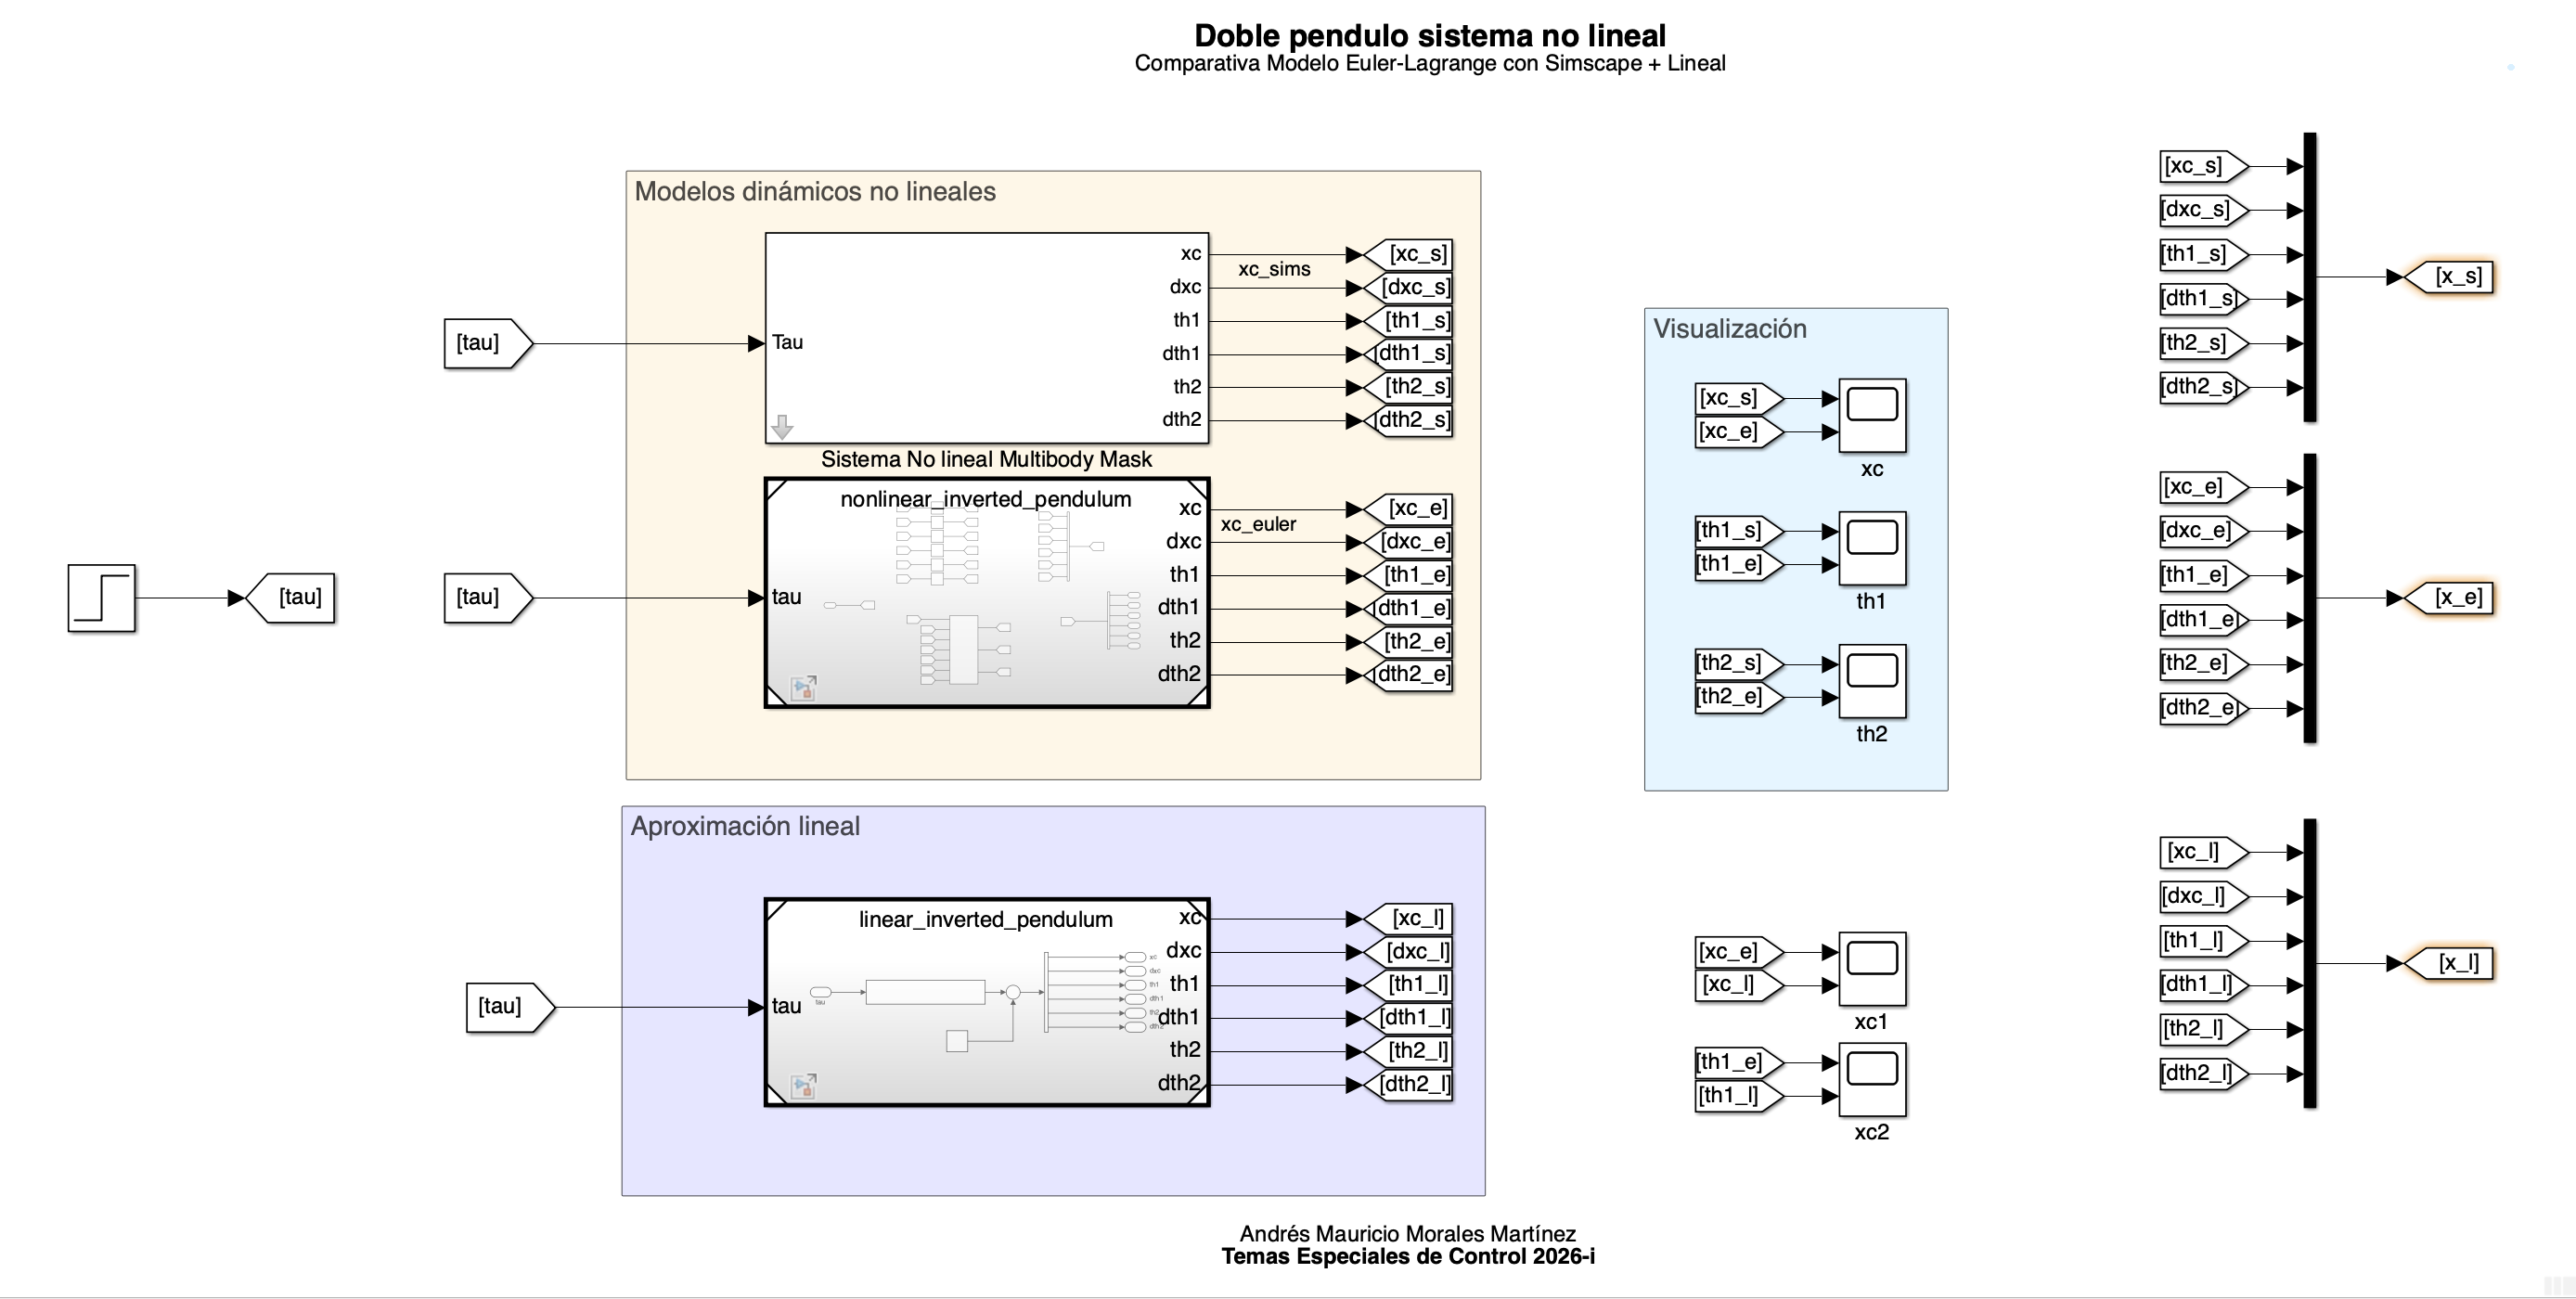
\includegraphics[width=\textwidth]{imgs/modelo/sistema_simulink_comparativa.png}
	\caption{Implementación en Simulink. Comparativa entre los tres modelos del sistema: modelo multicuerpo desarrollado en Simscape, modelo no lineal obtenido mediante Euler--Lagrange y modelo linealizado alrededor del punto de operación.}
	\label{fig:simulink_comparativa}
\end{figure*}

\begin{figure}[H]
\center
	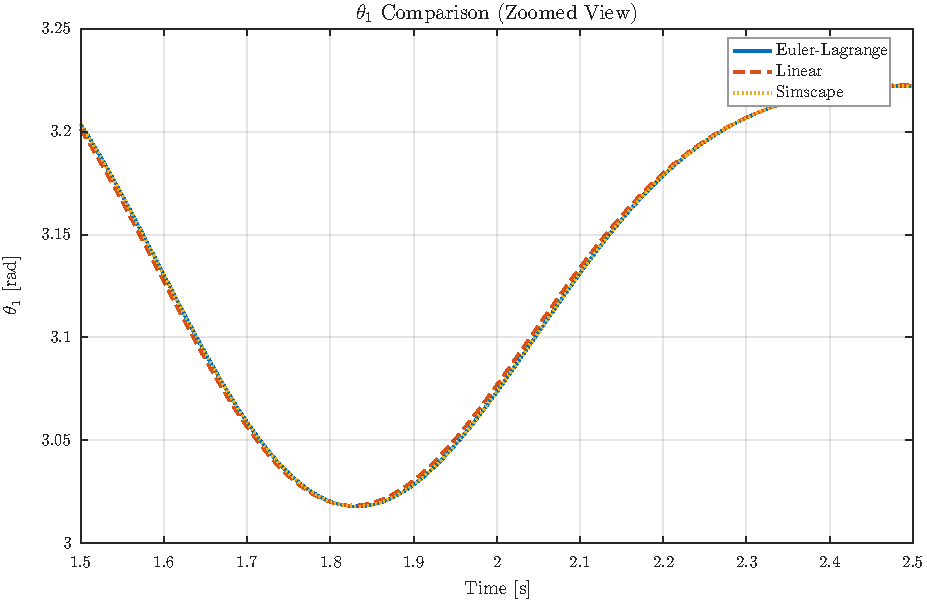
\includegraphics[width=0.8\linewidth]{imgs/modelo/zoomed_comparisson_responses.pdf}
	\caption{Tramo ampliado de $\theta_1$ para cada modelo implementado en Simulink.}
	\label{fig:comparativa_zoom}
\end{figure}

\begin{figure}[H]
\center
	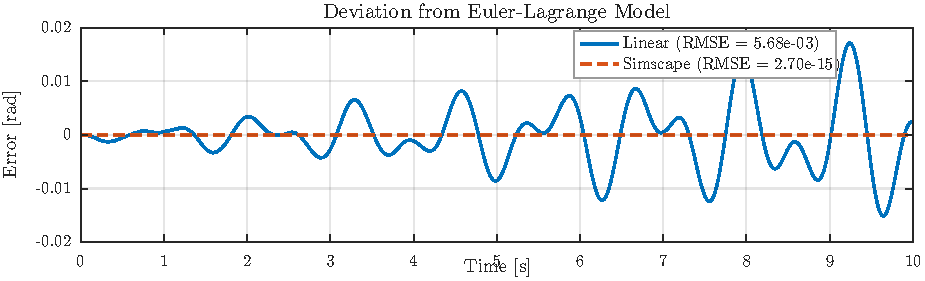
\includegraphics[width=0.8\linewidth]{imgs/modelo/error_overlap_responses}
	\caption{Error de la salida simulada respecto al modelo deducido mediante Euler--Lagrange.}
	\label{fig:error-comparativa}
\end{figure}


Como se evidencia en la Fig.~\ref{fig:comparativa_zoom}, la salida es muy similar para los tres modelos. No obstante, al observar el error (Fig.~\ref{fig:error-comparativa}), el modelo lineal presenta desviaciones que, aunque mínimas, son apreciables.\\

Es importante recordar que el modelo lineal sigue siendo una aproximación del sistema real; pese a la alta similitud en su respuesta, esta solo es válida en la vecindad del punto de operación. Incluso el modelo deducido mediante Euler--Lagrange omite dinámicas adicionales que sí pueden incluirse en el modelo multicuerpo de Simscape, tales como la rigidez de las articulaciones o el peso de las varillas de los péndulos. 
	
	\begin{figure}[H]
	\center
		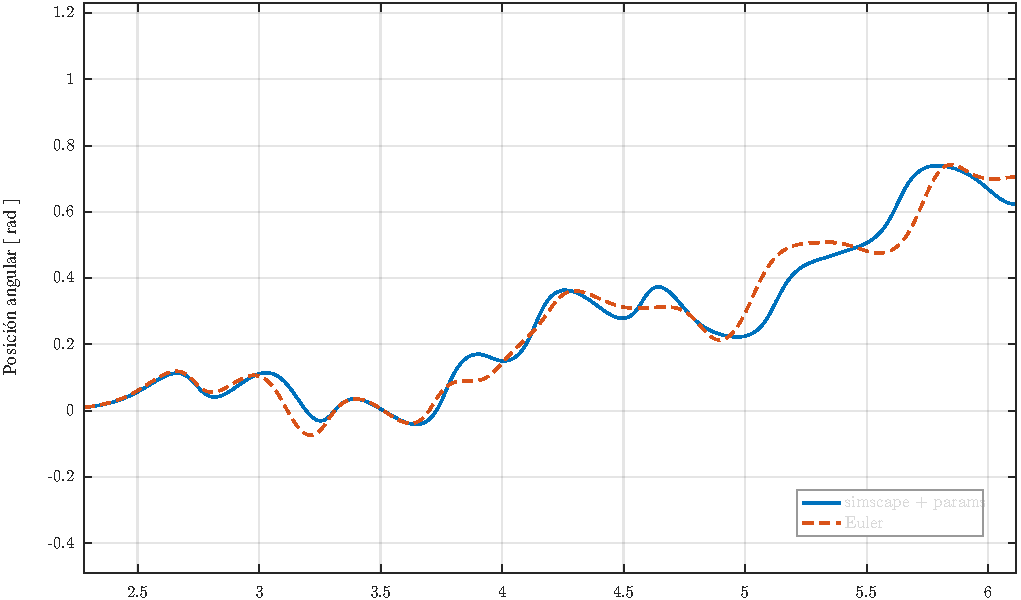
\includegraphics[width = 0.9\linewidth]{imgs/modelo/params_adds.pdf}
		\caption{Tramo ampliado de la comparativa de respuestas entre el modelo en Simscape y el modelo analítico por Euler--Lagrange. En Simscape se añade un amortiguamiento de $0.1$~N$\cdot$s/m al carro y de $0.3$~N$\cdot$m$\cdot$s/rad al péndulo 1.}
	\end{figure}
	
En la figura anterior se evidencia una clara variación en las respuestas, debida a los parámetros adicionales incorporados a la dinámica del modelo en Simscape que no fueron contemplados en el modelado analítico inicial.

El modelo no lineal de Euler--Lagrange se implementó en MATLAB despejando las aceleraciones generalizadas, como se muestra en el Listado~\ref{lst:fcn_dinamica}.

\begin{figure}[H]
\lstset{style=matlabstyle}
\begin{lstlisting}[caption={Función de MATLAB que implementa la dinámica no lineal del sistema, despejada para las aceleraciones generalizadas.}, label={lst:fcn_dinamica}]
function [ddxc, ddth1, ddth2] = fcn(tau, xc, dxc, ...
         th1, dth1, th2, dth2, parameters)
% Parametros
Mc = parameters.Mc;
m1 = parameters.m1;
m2 = parameters.m2;
l1 = parameters.l1;
l2 = parameters.l2;
g  = parameters.g;

den = -m1*cos(th1)^2 - m2*cos(th2)^2 + Mc + m1 + m2;

ddxc  = (l1*m1*sin(th1)*dth1^2 + l2*m2*sin(th2)*dth2^2 ...
         + tau - g*m1*cos(th1)*sin(th1) ...
         - g*m2*cos(th2)*sin(th2)) / den;

ddth1 = -(l1*m1*cos(th1)*sin(th1)*dth1^2 ...
         + l2*m2*cos(th1)*sin(th2)*dth2^2 ...
         + g*m2*sin(th1)*cos(th2)^2 ...
         - g*m2*cos(th1)*sin(th2)*cos(th2) ...
         + tau*cos(th1) - g*m1*sin(th1) ...
         - g*m2*sin(th1) - Mc*g*sin(th1)) / (l1*den);

ddth2 = -(l1*m1*cos(th2)*sin(th1)*dth1^2 ...
         + l2*m2*cos(th2)*sin(th2)*dth2^2 ...
         + g*m1*sin(th2)*cos(th1)^2 ...
         - g*m1*cos(th2)*sin(th1)*cos(th1) ...
         + tau*cos(th2) - g*m1*sin(th2) ...
         - g*m2*sin(th2) - Mc*g*sin(th2)) / (l2*den);
end
\end{lstlisting}
\end{figure}

\section{Salida plana}
Se busca plantear un controlador a partir del modelo lineal. Para ello se propone encontrar la salida plana del sistema. En el caso lineal, el procedimiento es análogo al método geométrico empleado en sistemas afines, pero se apoya en la matriz de controlabilidad.

Primero se recuerda que la matriz de controlabilidad $\mathcal{C}_{A,B}$ está dada por
\begin{equation}
	\mathcal{C}_{A,B} = \begin{pmatrix}
		B & AB & A^2 B & \cdots & A^{n-1} B
	\end{pmatrix},
\end{equation}
donde $n=6$ es el orden del sistema. Esta matriz contiene la información de cómo la entrada afecta a los estados. Si es de rango completo (no singular), se garantiza la controlabilidad del sistema. En el caso lineal, esto implica que existe una salida plana, ya que el sistema admite una forma canónica controlable.

A continuación se obtiene el vector $\lambda$ como la última fila de la inversa de la matriz de controlabilidad:
\begin{equation}
	\lambda^T = \begin{pmatrix}
		0 & 0 & 0 & 0 & 0 & 1
	\end{pmatrix}
	\mathcal{C}^{-1}_{A,B}.
\end{equation}

Con este vector se construye una matriz de transformación de estados $T$,
\begin{equation}
	T : X \to Z,
\end{equation}
que, aplicada sobre el vector de estados $x$, devuelve un nuevo vector $z$ asociado a la salida plana del sistema. Dicha transformación se define como
\begin{equation}
	T =
	\begin{pmatrix}
		\lambda^T \\
		\lambda^T A \\
		\lambda^T A^2 \\
		\vdots \\
		\lambda^T A^{n-1}
	\end{pmatrix},
\end{equation}
de modo que el cambio de coordenadas $z = Tx$ lleva al sistema a su forma canónica controlable. En estas nuevas coordenadas, la dinámica adopta la estructura de una cadena de integradores:
\begin{equation}
	\dot{z}_1 = z_2, \quad
	\dot{z}_2 = z_3, \quad \dots, \quad
	\dot{z}_{n-1} = z_n,
\end{equation}
\begin{equation}
	\dot{z}_n = \lambda^T A^{n} x + u.
	\label{eq:accion-control}
\end{equation}

\subsection{Acción de control}
Para el problema de seguimiento de trayectorias, conviene plantear el control respecto a la dinámica del error. Se define el error de seguimiento como
\begin{equation}
	e(t) = y(t) - y^*(t),
\end{equation}
donde $y^*(t)$ es la trayectoria de referencia que se desea imponer. Partiendo de la entrada $u$ dada por \eqref{eq:accion-control}, se propone la ley de control
\begin{equation}
	u(t) = -\lambda^T A^{n} x
	- \begin{pmatrix}
		k_0 & k_1 & \cdots & k_{n-1}
	\end{pmatrix}
	\begin{pmatrix}
		e \\ \dot{e} \\ \vdots \\ e^{(n-1)}
	\end{pmatrix}
	+ z^{*(n)}(t).
\end{equation}

Esta acción de control cumple tres funciones: (1)~cancela la dinámica interna del sistema mediante el primer término; (2)~impone una dinámica deseada sobre el error a través de la realimentación de estados; y (3)~introduce un término de prealimentación (\textit{feedforward}) basado en la derivada de orden $n$ de la referencia. En conjunto, esto permite realizar el seguimiento de la señal de referencia, cuya dinámica de error queda regida por
\begin{equation}
	k_0\, e + k_1\, \dot{e} + k_2\, \ddot{e} + \cdots + e^{(n)} = 0.
\end{equation}

Si los coeficientes $k_i$ se eligen de modo que el polinomio característico asociado sea Hurwitz, se garantiza la estabilidad del error y se pueden ubicar sus raíces (los polos del sistema en lazo cerrado) para obtener la respuesta temporal deseada.

Para este caso, se define el polinomio característico en el dominio de Laplace como
\begin{equation}
	\Delta(s) = (s + 5)^6.
\end{equation}
El polo real repetido en $s=-5$ asegura una respuesta Hurwitz con una rapidez moderada. Debido al orden elevado del polinomio, resulta preferible ajustar la ubicación de los polos por prueba y error en lugar de calcular analíticamente el tiempo de respuesta. No obstante, puede tomarse como referencia la constante de tiempo de una respuesta de primer orden, $\tau = 4/\sigma \approx 0.8$~s, teniendo en cuenta que el tiempo de establecimiento real será mayor debido a la multiplicidad del polo.

Los coeficientes $k_i$ se obtienen directamente a partir de los coeficientes del polinomio característico:

\begin{figure}[H]
\lstset{style=matlabstyle}
\begin{lstlisting}[caption={Cálculo de las ganancias de realimentación a partir de la ubicación de polos deseada.}, label={lst:ganancias}]
poles = [-5, -5, -5, -5, -5, -5];  % 6 polos en s = -5
p = poly(poles);                   % polinomio caracteristico
K_error = fliplr(real(p(2:end)));  % ganancias k_i
\end{lstlisting}
\end{figure}

Con los polos fijados, se implementó en Simulink la acción de control a partir de unas referencias sobre $z$, que describen la trayectoria que se desea seguir. La realimentación actúa sobre el error hasta $z_1^{(5)}$, mientras que la prealimentación toma la derivada faltante $z_1^{(6)}$ para alimentar el control de forma anticipada. Su implementación resulta relativamente sencilla gracias a la planitud diferencial, que parametriza la referencia en términos de la salida plana $z_1$ y sus derivadas.

\begin{figure}[H]
\center
	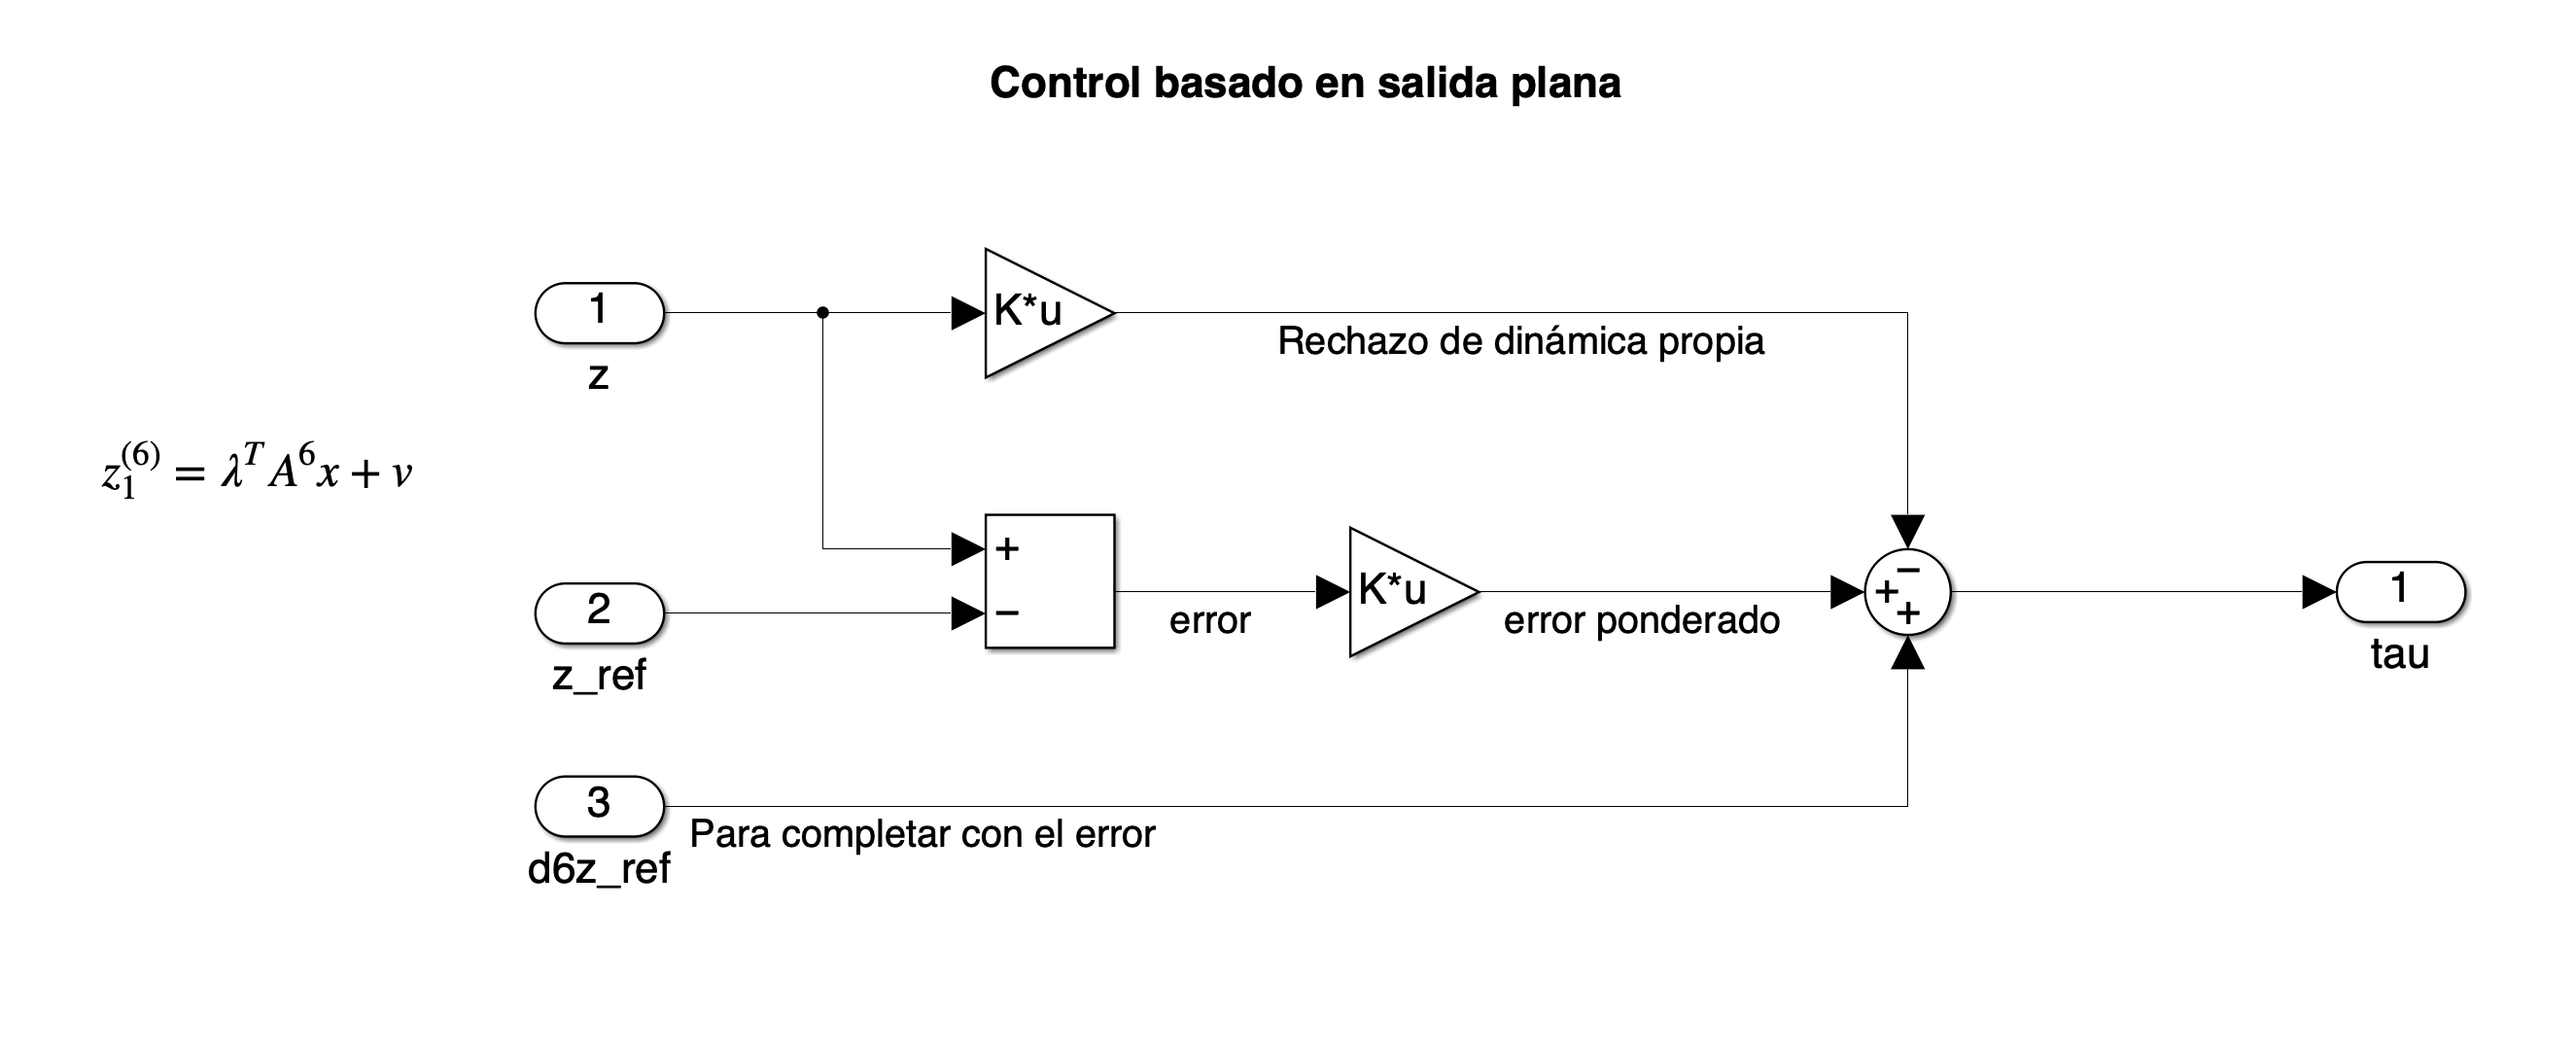
\includegraphics[width = 1\linewidth]{imgs/control/control-simulink.png}
	\caption{Implementación del control basado en salida plana. Suma del término de cancelación de la dinámica interna, la acción de realimentación (\textit{feedback}) y la acción de prealimentación (\textit{feedforward}).}
\end{figure}

Para la generación de las trayectorias se emplea el bloque \texttt{Ref Generator}. La trayectoria se suaviza hasta la quinta derivada y se define un tiempo final de $6$~s, partiendo de una posición inicial del carro de $-1$~m hasta una posición de referencia de $0$~m.

\begin{figure}[H]
\center
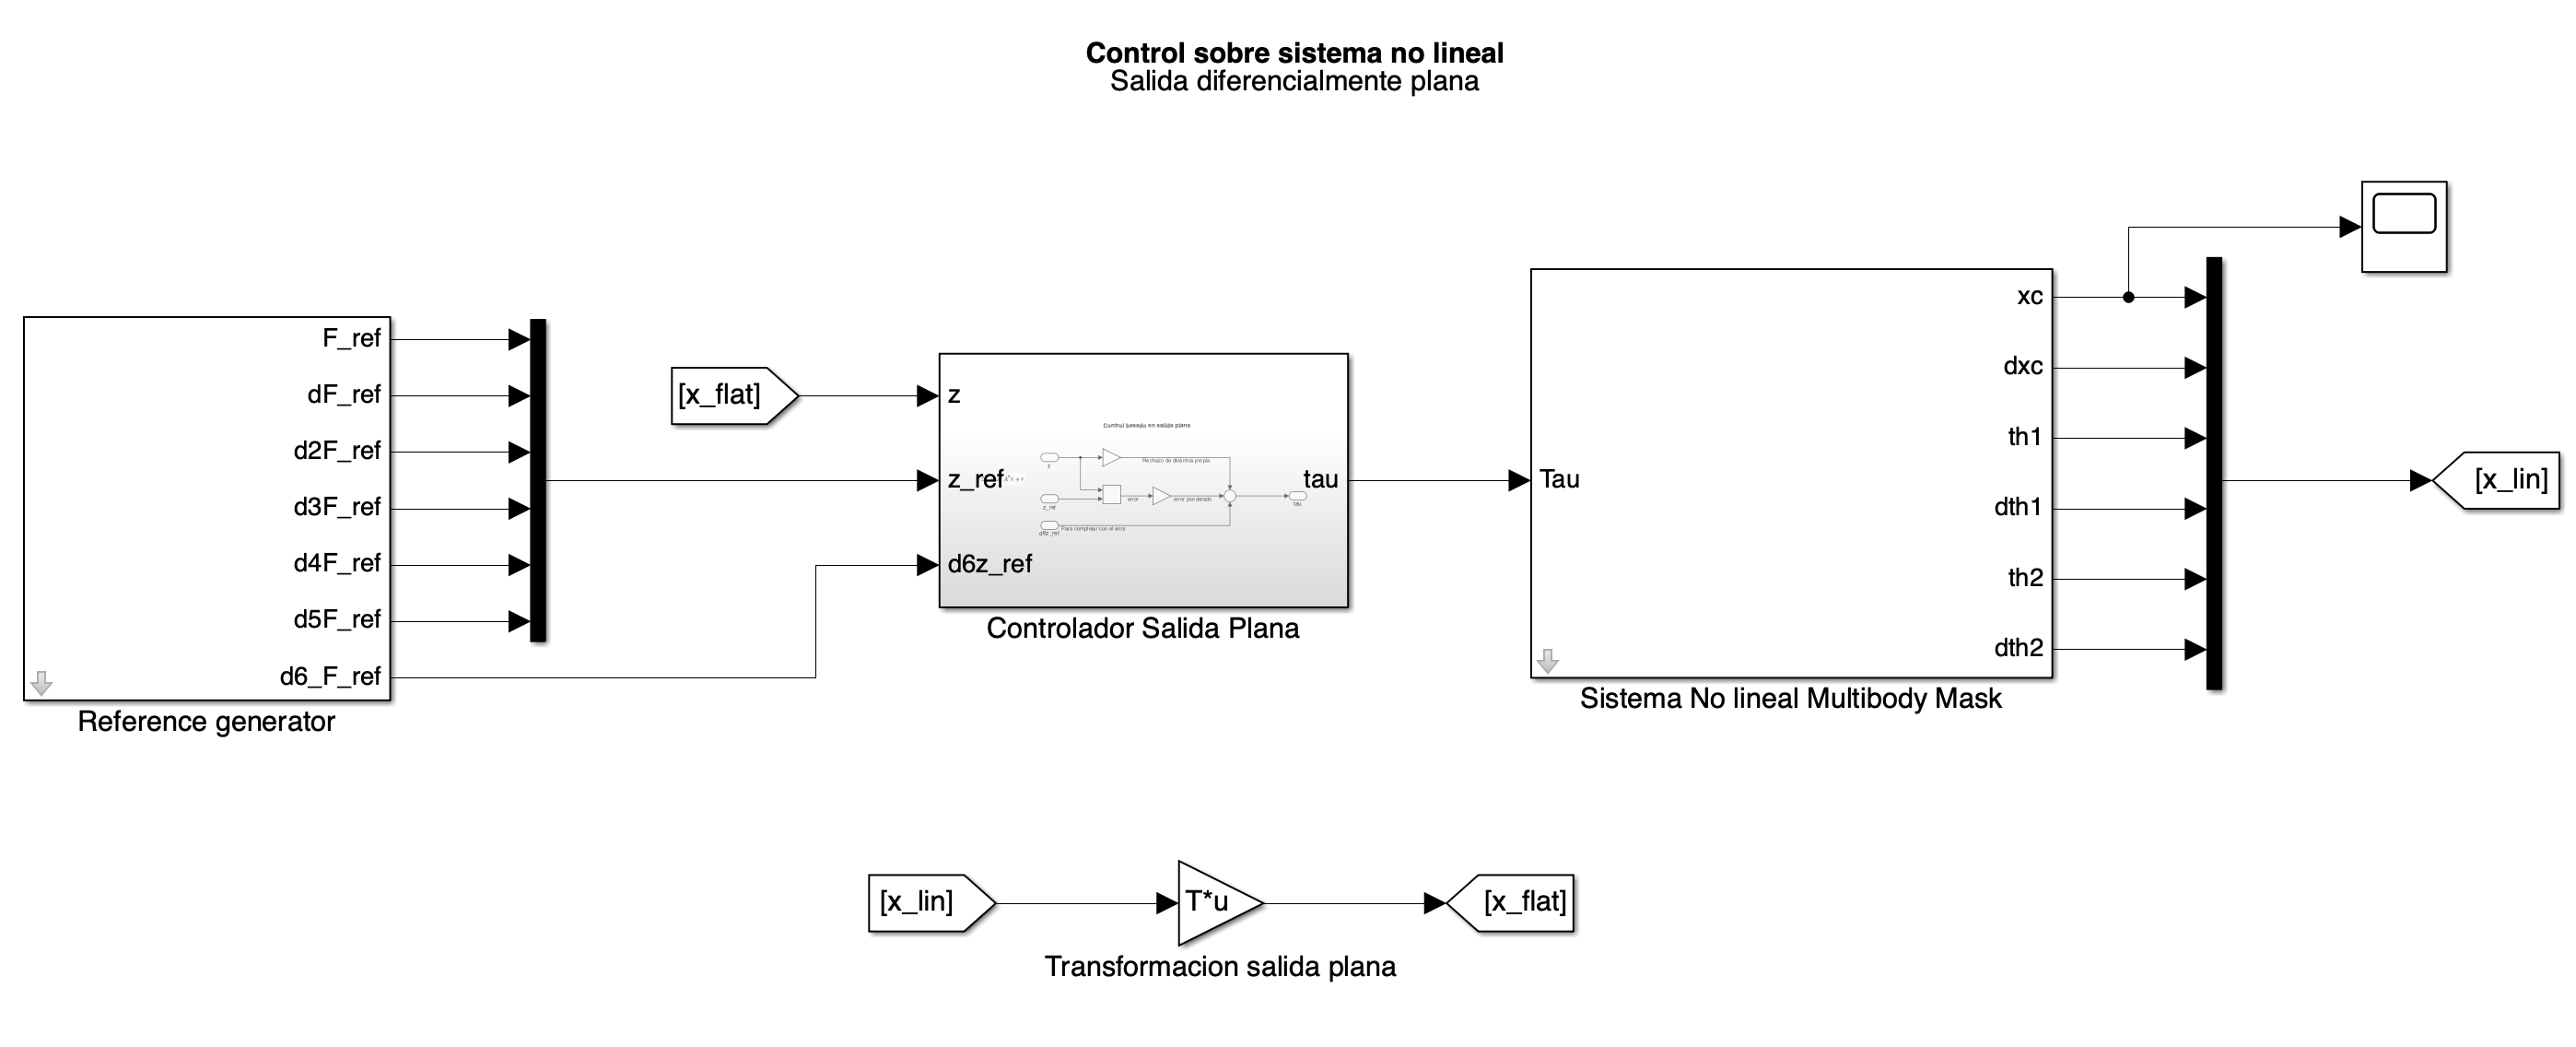
\includegraphics[width = 0.9\linewidth]{imgs/control/simulin-completo-control.png}
	\caption{Implementación completa del lazo cerrado para el problema de seguimiento sobre el sistema no lineal en Simscape Multibody.}
\end{figure}


\section{Resultados de control}
Se evaluó el desempeño del controlador basado en planitud diferencial ante cuatro conjuntos de condiciones iniciales, manteniendo constantes los parámetros del sistema y el punto de operación. La Tabla~\ref{tab:casos} resume las condiciones iniciales de cada caso, escogidas para abarcar distintas posiciones del carro y desviaciones angulares dentro del rango de validez del modelo lineal.

\begin{table}[H]
\centering
\caption{Condiciones iniciales para cada caso de simulación.}
\label{tab:casos}
\begin{tabular}{ccccccc}
\toprule
Caso & $x_c$ & $\dot{x}_c$ & $\theta_1$ & $\dot{\theta}_1$ & $\theta_2$ & $\dot{\theta}_2$ \\
 & [m] & [m/s] & [rad] & [rad/s] & [rad] & [rad/s] \\
\midrule
1 &  1.00 & $-0.01$ &  0.06 & $-0.05$ & $-0.08$ &  0.00 \\
2 & $-1.00$ &  0.01 & $-0.01$ &  0.03 &  0.04 & $-0.02$ \\
3 &  3.00 & $-0.10$ &  0.04 & $-0.05$ & $-0.01$ &  0.03 \\
4 &  4.00 &  0.01 & $-0.04$ &  0.05 &  0.03 & $-0.01$ \\
\bottomrule
\end{tabular}
\end{table}

En cada figura se muestra, de arriba hacia abajo, la acción de control, la posición del carro y la posición angular de los péndulos.

\begin{figure}[H]
\centering
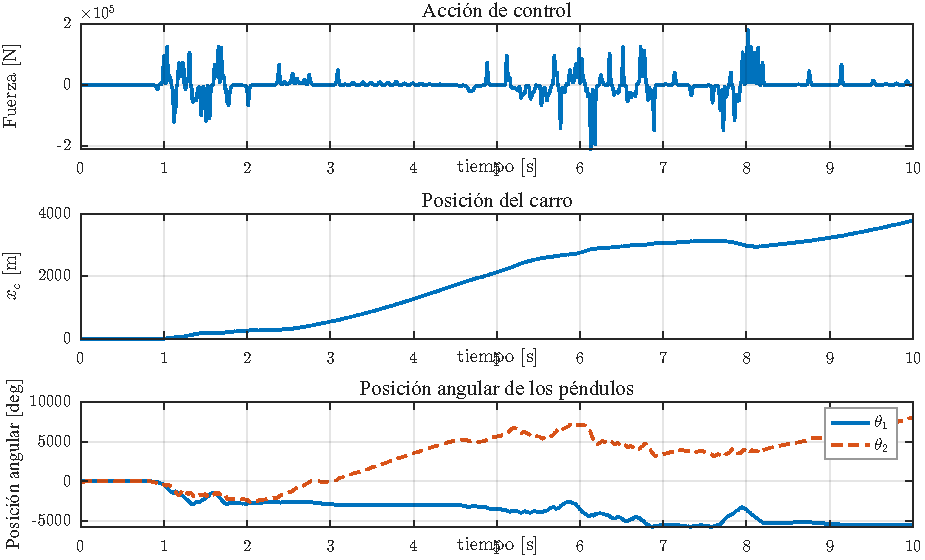
\includegraphics[width=0.9\linewidth]{imgs/control/control_case_1.pdf}
\caption{Respuesta del sistema en lazo cerrado para el Caso 1.}
\label{fig:caso1}
\end{figure}

\begin{figure}[H]
\centering
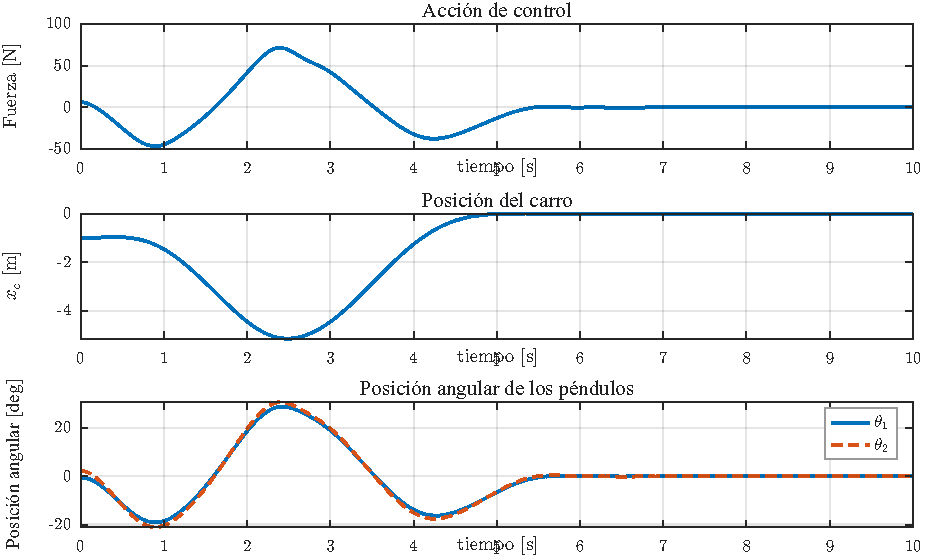
\includegraphics[width=0.9\linewidth]{imgs/control/control_case_2.pdf}
\caption{Respuesta del sistema en lazo cerrado para el Caso 2.}
\label{fig:caso2}
\end{figure}

\begin{figure}[H]
\centering
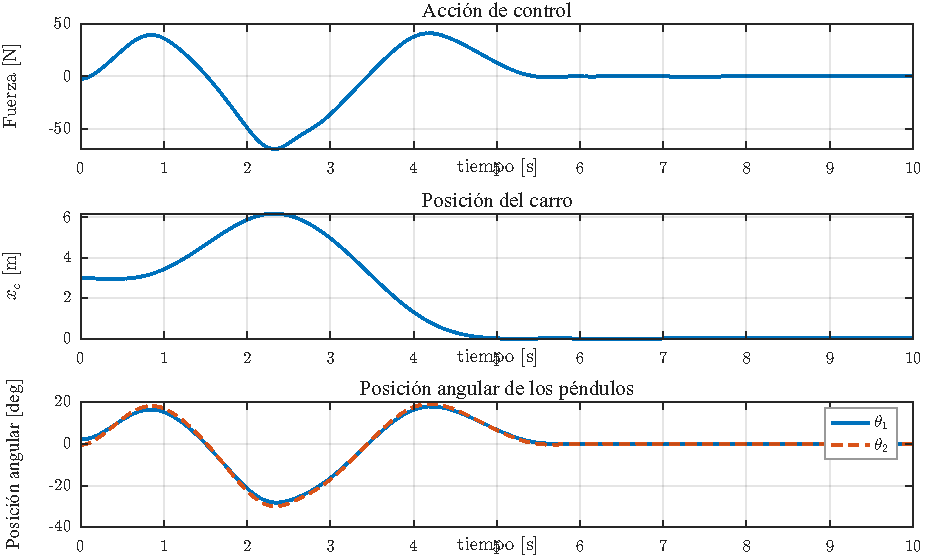
\includegraphics[width=0.9\linewidth]{imgs/control/control_case_3.pdf}
\caption{Respuesta del sistema en lazo cerrado para el Caso 3.}
\label{fig:caso3}
\end{figure}

\begin{figure}[H]
\centering
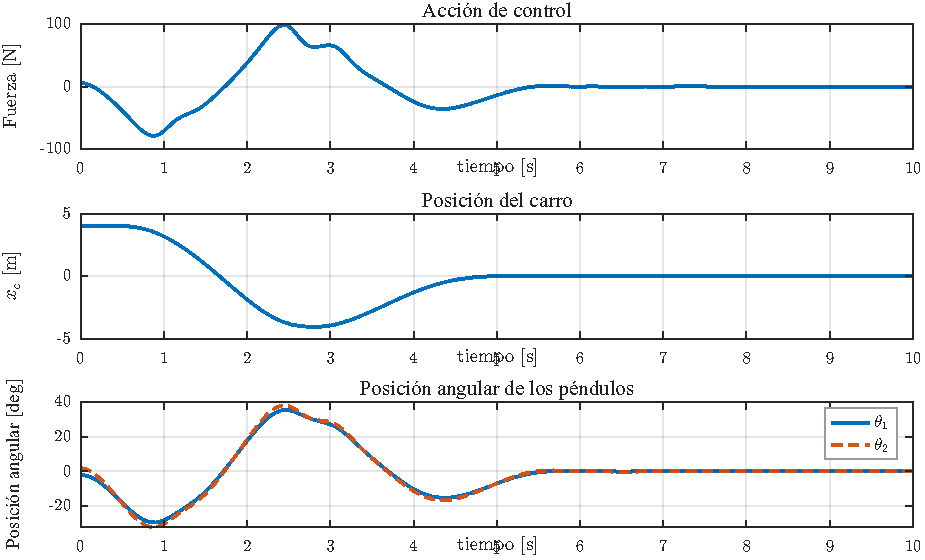
\includegraphics[width=0.9\linewidth]{imgs/control/control_case_4.pdf}
\caption{Respuesta del sistema en lazo cerrado para el Caso 4.}
\label{fig:caso4}
\end{figure}

Dado que la linealización se realizó en torno al equilibrio $q = (0,0,0,0,0,0)$, el control resulta válido únicamente en la vecindad de dicho punto. En el Caso~1, aunque la separación respecto al equilibrio no es muy grande, fue suficiente para desestabilizar la respuesta. En los Casos~2 y~4, la acción de control alcanzó magnitudes considerables, pero aun así se logró estabilizar el sistema; de los cuatro, el Caso~2 fue el más estable. Estos resultados evidencian la limitación de trabajar sobre un sistema linealizado de forma local, en contraste con un enfoque de validez global como el que ofrecería una linealización por realimentación.

\subsection{Perturbación}
Se propone una perturbación simple sobre la masa~2: en $t = 3$~s se aplica una fuerza horizontal de $F = 5$~N. Por ahora se consideran únicamente los Casos~2, 3 y~4 del análisis anterior, por tratarse de condiciones estables.

\begin{figure}[H]
\centering

\includegraphics[width=0.9\linewidth]{imgs/control/perturbacion/control_case_1.pdf}
\caption{Respuesta del sistema ante perturbación para el Caso 2.}
\label{fig:pert_caso2}
\end{figure}

\begin{figure}[H]
\centering

\includegraphics[width=0.9\linewidth]{imgs/control/perturbacion/control_case_2.pdf}
\caption{Respuesta del sistema ante perturbación para el Caso 3.}
\label{fig:pert_caso3}
\end{figure}

\begin{figure}[H]
\centering

\includegraphics[width=0.9\linewidth]{imgs/control/perturbacion/control_case_3.pdf}
\caption{Respuesta del sistema ante perturbación para el Caso 4.}
\label{fig:pert_caso4}
\end{figure}

En el Caso~3, la perturbación desestabilizó la respuesta. En cambio, los Casos~2 y~4 lograron resistir la perturbación, mostrando una buena robustez.

\section{Conclusiones finales}
\begin{itemize}
    \item El formalismo Lagrangiano permite modelar sistemas complejos con relativa facilidad, en comparación con el enfoque de Newton--Euler. No obstante, un modelo es tan bueno como sus suposiciones iniciales: si se omiten dinámicas reales o parámetros propios del sistema —tales como la rigidez, la inercia aparente de elementos adicionales o el amortiguamiento—, se obtiene un modelo que no refleja con exactitud el problema real. Por ello, debe buscarse un equilibrio entre la exactitud del modelo y la complejidad del problema, confiando en el control como mecanismo de robustez para que un modelo aproximado resulte suficiente como referencia para el diseño del compensador.

    \item La salida plana es una técnica de geometría diferencial que permite parametrizar el sistema en términos de una única salida y sus derivadas. Esto facilita la tarea de control por seguimiento, ya que la parametrización incorpora la referencia de forma natural y permite alimentar la ley de control casi directamente a partir de dicha referencia.

    \item Al realizar el control sobre un sistema linealizado, es importante notar que no se garantiza estabilidad global, sino únicamente un funcionamiento local. Este enfoque simplifica considerablemente el diseño del controlador, pero puede no ofrecer las prestaciones de robustez global deseables en problemas reales; de hecho, su rango de acción puede llegar a ser bastante limitado. Como extensión, es posible explorar la linealización por realimentación (\textit{feedback linearization}) para ampliar la región de operación más allá de la vecindad del punto de aproximación.

    \item En conjunto, el control permite imponer la dinámica deseada sobre un sistema altamente no lineal a partir de una linealización sencilla. Si bien existen limitaciones evidentes, estas no restan valor al control por salida plana ni a su notable capacidad de simplificación.
\end{itemize}




\end{document}